\documentclass[a4paper,oneside,11pt]{book}

\usepackage{NWUStyle}
\usepackage{bibentry}
%================================================================================

\begin{document}

\Title{The viability of post-graduate students developing a commercial ERP system of industry standards: A South African Case Study}
\Initials{J. F.}
\FirstName{Franco}
\Surname{Du Plessis}
\StudentNumber{33642958}
\ORCID{placeholder}
\MScorPhD{Magister Scientiae} 
\Field{Computer Science} 
\GradDate{2025}
\Supervisor{Prof. C. J. Kruger}
\CoSupervisor{} 
\AssistantSupervisor{} 
%---------------------------------------------

\MakeTitle 

%-------------------EDIT----------------------
%Type your acknowledgements:
\begin{Acknowledgements}{}
			I would like to thank the everyone for helping me. You're all great!
\end{Acknowledgements}
%---------------------------------------------

%-------------------EDIT----------------------
%Type your abstract:
\begin{Abstract}{}
			This is the abstract. It is a summary of all the work.
			%Provide all of your keywords here (separated by semi-colons. This will appear below the abstract.
			\KeyWords{Keyword 1; Keyword 2; Keyword 3.}
\end{Abstract}
%---------------------------------------------

\MakeTOCandLOFandLOT %This command creates the table of contents, list of figures and list of tables.

%-------------------EDIT----------------------
%[OPTIONAL] Type your table of abbreviations. Delete this if you do not intend to use it.
\begin{TableOfAbbrev}
			A table containing a list of abbreviations that will be used throughout text.
			\begin{table}[!htpb!]%
			\begin{tabular}{ll}
			\textbf{ERP} & Enterprise Resource Planning\\
                \textbf{CRM} & Customer Relationship Management\\
                \textbf{DSR} & Design Science Research\\
                \textbf{IS} & Information Science\\
                \textbf{CR} & Critical Realism\\
                \textbf{ADR} & Action Design Research\\
			\end{tabular}
			\end{table}
\end{TableOfAbbrev}
%---------------------------------------------

\pagestyle{headings}
\setcounter{page}{1}
\pagenumbering{arabic}

%================================================================================
%BEGIN TYPING YOUR DOCUMENT - STARTING HERE.-------------------------------------
%================================================================================
\chapter{Introduction}
\par{The demand for efficient and adaptable enterprise solutions has never been greater in today's
rapidly evolving technological landscape. Within the South African context, where the
intersection of academia and industry holds significant promise for innovation and economic
growth, the exploration of novel approaches to software development becomes imperative. This
introduction outlines the rationale, objectives, and structure of the research study aimed at
investigating the feasibility and efficacy of leveraging university student talent to develop a
commercial-grade software solution in the form of an Enterprise Resource Planning (ERP)
system in collaboration with TaskFlow a partnering North-West University-industry software
development company.}

\par{Collaboration between industry and academia is essential to benefit the global technological
village \citep{baig2018bridging}. Unfortunately, universities, especially in developing nations, often lack the resources to allow for the proper development of skills needed by students entering the software development workforce. Through collaborative initiatives, software companies possess
the necessary skills, know-how, and technology to improve the skills of university students in a
controlled environment that simulates real-world experience. For instance, companies
specialising in software development, like TaskFlow, integrate solutions such as Contact Centre,
Customer Relations Management, Dialer, and Helpdesk into a comprehensive Enterprise
Resource Planning (ERP) suite. This empowers their clients to optimise time and make
informed business decisions through tailor-made and integrated software that more efficiently
and effectively streamlines their entire business processes.}

\par{Integrated ERP systems significantly affect the organisation's value chain in both primary and secondary operations \citep{amini2020erp}. By connecting business and management
activities, enterprise resource planning (ERP) assists organisations in realising their full potential \citep{uccakturk2013effects}. Additionally, while ERP systems are pivotal to operational
success, the associated expenses of non-integrated software solutions present significant barriers
to cost and scalability. Consequently, many software-developing companies aim to minimise the
cost of training interns on the theory behind and use of integrated software tools, project management, and software development, especially when developing complex systems such as ERP suits. This research aims to investigate whether Higher Education Institutions (HEIs) can effectively address the current challenges faced by the industry by introducing collaborative
university/industry-applied teaching to some postgraduate computer science and information
systems curricula. By doing so, the study explores the viability of creating a mutually beneficial
relationship between academia and industry, which can bring positive outcomes for both parties and students. As such, the research will delve into the potential of the curricula in Project management and System development at Honor's level to mitigate the challenges faced by the
industry while nurturing a dynamic and symbiotic partnership between academia and industry.}

\section{Problem Statement}
\par{The intersection of academia and industry presents unique opportunities and formidable
challenges. Employers find it challenging to locate people with the knowledge and abilities
needed for open positions \citep{barnett2011partnering}. Former President Barack Obama thus emphasised the need for lawmakers and national higher education associations to urge educational institutions to not only set ambitious educational attainment targets but also ensure that their goals address the current gap in required industry skills \cite{barnett2011partnering}. Thus, creating an educational environment for efficient learning and skill development is imperative to provide the correct skills for industry \citep{baig2018bridging}. Therefore, it is beneficial for graduate students to comprehend how the industry operates and how idea and innovation are turned into the products and services society requires \citep{foley1997technology}.}
\par{The central inquiry for this study emerges from the argument that tertiary education students
need to be trained for the requirements of a professional workspace \citep{baig2018bridging}. The
question arises: \textit{To what extent can postgraduate students be effectively taught to
develop industry-standard software solutions such as ERP systems amidst the multidimensional challenges of technical proficiency, client satisfaction, and academic rigour?}}

\section{Research Aims and Objectives}
\par{The upcoming study will concentrate on three primary objectives. First, it will define the essential components and prerequisites of a fully functional, versatile, and industry-approved software system. Secondly, it aims to pinpoint the critical abilities that students must possess to create an acceptable software system in the industry. Lastly, it will explore the roles of academia and industry in facilitating the successful creation of such a system through sound project management and system development skills.}
\par{This study aims to evaluate the feasibility of creating a commercially viable software solution in
collaboration with a software development company as part of the NWU computer science and information systems department's prescribed curriculum on IT project management and software development honours program. Through collaboration with the industry, this study aims to showcase the technical abilities of computer science students by developing a software solution that meets commercial standards. This initiative also seeks to equip students with the necessary skills to become valuable contributors to the South African workforce. The project aims to conduct a pilot study to identify the key success factors in guiding postgraduate students at a Higher Education Institution (HEI) in an underdeveloped country. The goal is to provide these students with industry exposure in a formalised academic and learning environment, enabling them to develop economically viable software. The study seeks to determine how the students can be effectively mentored and trained and what support and resources are necessary to ensure their success.
Ultimately, the findings of this study will be used to inform the design of future programs that seek to foster innovation and economic growth in underdeveloped regions of the world.}
\par{This study explores the possibility of integrating projects and software development techniques taught in an educational setting by teaching existing structures and practices of a typical software development company in the South African industry. The objective is, therefore, to teach computer science and information systems graduates to identify market opportunities and, by applying industry practices and sound PM and SD methods, to develop software products that are commercially viable and aligned with market demands. As such, the research seeks to uncover optimal practices and tactics that improve educational insights regarding the teaching of PM and software development procedures, integrating cutting-edge best practices from the industry. To assess the software solution's viability as a marketable product, the research will conclude through an extensive evaluation by proficient experts and professionals in the software development industry. It will also involve thoroughly examining the client's satisfaction and feedback after receiving the final system, including any concerns they may raise. This
assessment will determine the critical success factors in developing commercial software, the roles of industry and academia in the learning process, and any necessary improvements to enhance the learning experience.}

\section{Hypothesis}
\par{Postgraduate computer science and information systems students can build a sophisticated software solution that is commercially viable, such as an ERP system when partnering with the expertise and resources of industry partners.}

\section{Methods of Investigation}
\par{Throughout the commencement of the research, the study will draw upon two main facets to substantiate the claims made in the paper's conclusions: the vast amount of academic literacy available and the other experiment based data collection processes referring to the development project as the main experiment. Both of these will be outlined below to provide clarity on both matters.}
\subsection{Literature Study}
\par{To enhance the credibility, accuracy, and validity of the study, a thorough and systematic review of pertinent literature will be conducted. This will involve targeting keywords such as higher education, academia, ERP systems, software success, project management, system implementation, and commercialisation. Research will be prioritised from a positivist perspective and examine peer-reviewed articles from reliable sources such as the NWU Library, Google Scholar, IEEE Xplore, and ACM Digital Library. In addition, grey literature from trusted sources like white papers and industry reports will be considered, as this research incorporates best practices from the industry. Duplicate articles or those not meeting our eligibility criteria will not be accepted. To locate important material, references from key papers will be scrutinised and analysed for citation patterns, thus seeking advice and insights from
subject matter experts. The focus will be on resources published between 2015 and 2024 to ensure relevance. Historical research to be focused on include:}
\par{\begin{itemize}
    \item Njanka, S. Q., Sandula, G., and Colomo-Palacios, R. (2021). It-business alignment: A
systematic literature review. Procedia Computer Science, 181:333–340.
    \item Kenge, R. and Khan, Z. (2020). A research study on the erp system implementation and
current trends in erp. Shanlax International Journal of Management, 8(2):34–39.
    \item Guo Chao Alex, P. and Chirag, G. o. C. I. S. (2014). Cloud erp: a new dilemma to modern
organisations? Journal of Computer Information Systems, 54(4):22–30.
    \item Bagchi-Sen, S., Baines, N., and Smith, H. L. (2022). Characteristics and outputs of univer-
sity spin-offs in the united kingdom. International Regional Science Review, 45(6):606–
635.
\end{itemize}}
\subsection{Methods of Investigation}
\par{As mentioned earlier, this study aims to thoroughly examine the literature on software systems and student development of software in developed nations to identify applicable lessons for developing environments like South Africa. A key objective is to equip students with the knowledge needed in PM and system development to create software that adheres to industry best practices. To achieve this, the study will assess the business case for higher educational institutions to develop commercially viable software for the industry as potential clients. Once
the need is established, the next step will be identifying the technological and functional requirements for creating software that real-world clients can use to support their daily operations. Once the software is completed, the study will evaluate the usability of the software as well as the learning experience and the proficiency of postgraduate students in applying project management and systems development methodologies to complex software development. The aim is to offer significant and insightful knowledge that can be utilised by higher education institutions (HEIs) in underdeveloped countries to improve the functionality, efficiency, and acceptance of their software and systems development projects. This will help HEIs teach the most relevant and useful theories of project management and teamwork, ultimately enhancing their students employability and marketability in the industry.}
\par{As such, the researcher will serve as an integral part of the project, overseeing software development. As mentioned, according to set project management milestones, the software system will undergo testing by reviewers with experience in the information technology and ERP industries. All lessons learned and the input from reviewers will be compiled to produce a workable framework that can direct HEIs in leveraging project management and software development curricula to develop commercially viable software solutions and systems for internal and industry applications.}

\section{Chapter Division}
\par{This thesis is structured into six main chapters, each meticulously crafted to delve into specific
facets of the research endeavour, elucidating methodologies, literature insights, empirical findings, and concluding reflections. The chapters are as follows:}
\par{The Research Design chapter serves as the foundational cornerstone of the thesis, this chapter
provides a detailed exposition of the research methodology and paradigm guiding the study. Adopting a design science research methodology and a positivist paradigm, this section navigates the theoretical underpinnings of the research approach, outlining its epistemological and ontological foundations. Through meticulous delineation of research
methods, including data collection techniques, sampling strategies, and analytical frameworks, this chapter lays the groundwork for subsequent empirical inquiry. Once this chapter has concluded, a review of the current literature in the field will be done to pinpoint previous scientific findings that will benefit the current study.}
\par{The Literature Study chapter embarks on an immersive journey through the annals of academic literature, traversing diverse domains ranging from ERP systems to implementation frameworks. The section unfolds with a lucid articulation of the problem statement, contextualising the research within the broader academic discourse. Subsequent sections delve into the intricacies of ERP systems, exploring their architectural nuances, functional capabilities, and strategic significance within organisational contexts. Furthermore, the chapter probes into the value chain framework, dissecting the interconnected dynamics of people, processes, and technology in driving organisational success. Anchored by comprehensive reviews of commercialization strategies, software implementation frameworks, and the role of students in industry, this chapter serves as a beacon of scholarly inquiry, illuminating the theoretical landscape underpinning the research endeavor. Once the theoretical landscape has been illuminated, a case study can be conducted to generate findings regarding the research question, and help the research endeavour edge closer to final conclusion.}
\par{The Case Study embarks on a voyage of empirical exploration, this chapter unfurls the intricacies of the case study conducted within the hallowed confines of TaskFlow. With a keen focus on project design and execution, this section unveils the methodological blueprint guiding the project life cycle. Through an exhaustive examination of project management methodologies, agile development frameworks, and strategic planning processes, this chapter offers unparalleled insights into the operational dynamics underpinning software development endeavours. Furthermore, by delineating the project pipeline and process, this section charts the trajectory of the project's evolution, elucidating key milestones, challenges encountered, and lessons learned along the way. Once the case study has concluded, and sufficient data is collected around the subject at hand, an expert reviewer will reveal the depth of the truth within the findings and help the project reach its final conclusion.}
\par{In pursuit of academic rigour and scholarly validation, the Expert Reviewer chapter invites the discerning gaze of domain experts to scrutinise the research methodology and findings. Through structured interviews, expert assessments, and critical appraisals, this section seeks to engender a dialectic discourse, fostering intellectual exchange and epistemic enrichment. By subjecting the research endeavour to rigorous scrutiny, this chapter endeavours to enhance the robustness and validity of the research findings, ensuring their salience and applicability within the broader academic community. The chapter that follows will discuss the results that were found throughout the study.}
\par{The Results and Discussion serves as the crucible of empirical inquiry, this chapter presents and analyses the empirical findings gleaned from the case study and expert review. Through meticulous data analysis techniques, including qualitative coding, thematic analysis, and comparative synthesis, this section unveils the rich tapestry of insights garnered from the research endeavour. Furthermore, by fostering a dialectic discourse between empirical findings and theoretical frameworks, this chapter endeavours to unravel the underlying mechanisms and causal relationships shaping the research phenomena. The chapter that follows will make the final conclusions regarding the total study and its findings; it will act as a summary for the research project and summarise the findings to draw the final conclusion.}
\par{The conclusions chapter aims to synthesise key insights, implications, and avenues for future research, this chapter offers a reflective denouement to the research endeavour. Through a judicious synthesis of empirical findings and theoretical frameworks, this section distils the essence of the research inquiry, elucidating its broader implications and relevance within academic and practical contexts. Furthermore, by delineating avenues for future research and scholarly inquiry, this chapter seeks to catalyse intellectual curiosity and foster a culture of continuous learning and innovation.}
\par{In summation, this research endeavour represents a concerted effort to bridge the gap between academic theory and industrial practice, laying the foundation for the subsequent chapter, "Research Design." By elucidating the theoretical underpinnings and methodological frameworks guiding the study, the forthcoming chapter endeavors to translate lofty aspirations into tangible research methodologies, fostering innovation, collaboration, and economic prosperity within the South African software development landscape.} 
\chapter{Research Design}
\par{This chapter outlines the research design employed to in the study. The aim is to investigate and reveal the most optimal research methodology and paradigm that encourage the success of the case study. The methodology encompasses Design Science Research (DSR) within the positivist paradigm, emphasising the creation and evaluation of innovative artefacts to address specific challenges. Data collection will primarily involve monitoring a case study, supplemented by interviews with experts, with analysis conducted through quantitative methods.}
\par{The following chapter will explore and pinpoint areas of relevance to the study within the domain of research design. The chapter begins by examining various research methodologies relevant to the field and discussing the chosen methodology to be used in greater depth, addressing the relevant literature and the effect these findings will have on the research project at hand. The same exploration is then done on research paradigms and which will be most suitable and fitting for the current study, concurrently addressing the affect the choice will have on the research project. The chapter then continues to delve into methodologies for determining the success of completion of the artefact and makes use of that information to determine what data collection will be done so that a quantitative conclusion can be made at the end of the study. The rest of the chapter defines how the research is designed and how it will be conducted, as well as how ethical clearance is acquired and what ethical implications the project could have.}


\section{Exploring Research Methods using the Research Onion}
\par{When doing research, the research onion created by \cite{saunders2009research} is frequently used as a design guide. A growing number of researchers from different disciplines are increasingly embracing the research onion model as a basis for their study design, despite its original primary use in business research. The layers of the research onion represent several aspects of formulating a research strategy, the outer layers are more theoretical and the interior levels more practical \citep{saunders2009research}. The figure below shows the research onion that was outlined by \cite{saunders2009research}.}
\begin{figure}[h!]
    \centering
    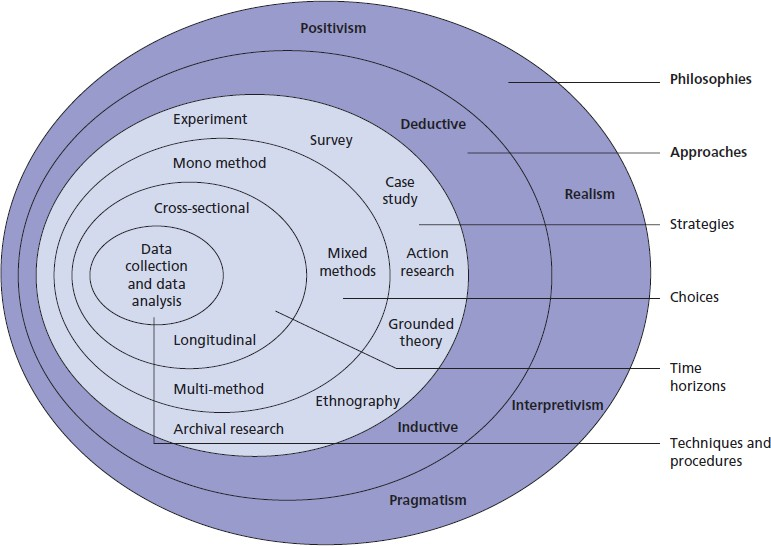
\includegraphics[width=1\linewidth]{img/Saunders research onion.jpg}
    \caption{The Saunders Research Onion}
    \label{fig:enter-label}
\end{figure}
\par{Since IS is a field of study that integrates both the natural and social sciences, employing the research onion as proposed by \cite{saunders2009research} in and of itself requires some adjustments as it has not yet taken into account all the techniques and strategies used in the field of IS. Therefore, \cite{mardiana2020modifying} proposed a modified version of the research onion that is more catered towards the field of information science research. The modified version of the research onion can be seen in the figure below.}
\clearpage
\begin{figure}[h!]
    \centering
    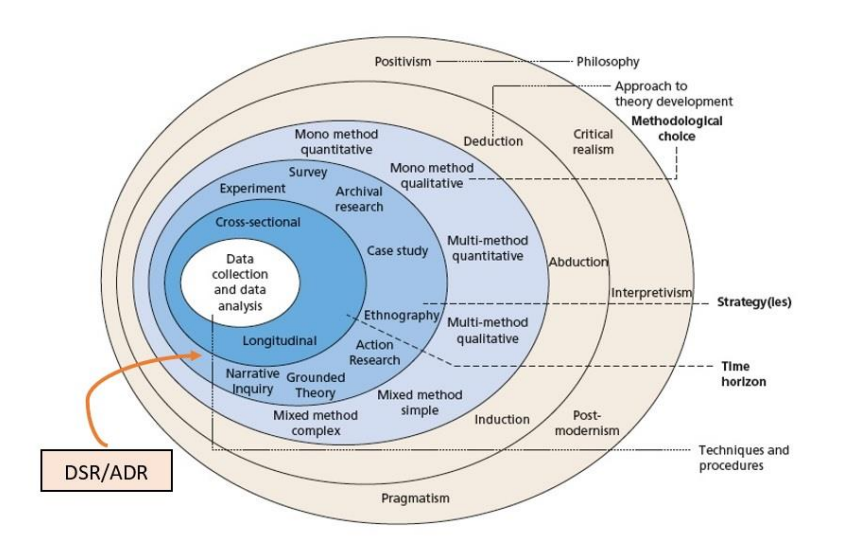
\includegraphics[width=1\linewidth]{img/Modified research Onion.png}
    \caption{The Modified Research Onion}
    \label{fig:enter-label}
\end{figure}
\par{As it is some what difficult to understand the implications of the modified research onion, \cite{mardiana2020modifying} also provides the following table showing how research design can be constructed by making use of the modified research onion.}
\begin{table}[h!]
\centering
\small 
\begin{adjustbox}{max width=\textwidth}
\begin{tabular}{|p{2.2cm}|p{2.2cm}|p{2.2cm}|p{2.2cm}|p{2.5cm}|p{2.5cm}|}
\hline
\textbf{Philosophy} & \textbf{Approach} & \textbf{Methods} & \textbf{Strategy} & \textbf{Time horizon} & \textbf{Data collected} \\
\hline
Positivism & Deductive & Quantitative & Experiment & Cross-sectional Longitudinal & Numerical \\
\hline
Positivism & Deductive & Quantitative & Survey & Cross-sectional Longitudinal & Numerical \\
\hline
Interpretivism & Inductive & Qualitative & Archival research & Cross-sectional & Non-Numerical \\
\hline
Interpretivism & Inductive & Qualitative & Case study & Cross-sectional & Non-Numerical \\
\hline
Interpretivism & Inductive & Qualitative & Ethnography & Cross-sectional & Non-Numerical \\
\hline
Interpretivism & Inductive & Qualitative & Action Research & Cross-sectional & Non-Numerical \\
\hline
Positivism Interpretivism Pragmatism & Abductive Deductive & Quantitative Qualitative & Design research & Cross-sectional Longitudinal & Numerical Non-Numerical \\
\hline
Interpretivism & Inductive & Qualitative & Grounded theory & Cross-sectional & Non-Numerical \\
\hline
Interpretivism & Inductive & Qualitative & Narrative inquiry & Cross-sectional & Non-Numerical \\
\hline
\end{tabular}
\end{adjustbox}
\caption{The possible research design composition in IS research}
\end{table}
\par{The research onion and its recommendations will be used to construct the research design that will be employed by this research project, as it provide guidelines for which options of the various components of research align with one another and are well suited. Each component of research, namely philosophy, approach, methods, strategy, time horizon, and date collected, will be further researched and investigated throughout the rest of this chapter in order to define the complete design of the research project.}


\section{Research Philosophy}
\par{A research philosophy explains the study's methods and the type of knowledge that was produced, as well as the researcher's viewpoint on the relationship between knowledge and development. The subsections that follow outline the various philosophies that form part of the modified research onion created by\cite{mardiana2020modifying}. Each philosophy will be studied independently in order to determine the viability of the outlook in the context of the research being conducted.}
\subsection{Positivism}
\par{Philosophers Descartes and Locke served as major influences during the 17th and 18th century Enlightenment, which is when positivism first emerged \citep{park2020positivism}. Over time, logical positivism also began to emerge. The idea that there is a universal, temporal truth that all disciplines must adhere to is greatly influenced by logical positivism, which holds that although scientific laws frequently emerge through the use of intuition, this does not entail that the laws can be subjectively justified \citep{luczak2013beyond}. Moreover, logical positivism's theory of truth consists of providing a solution to the following query: "For every given statement p, what are the conditions under which p (is true) and what are the conditions under which not-p?". Therefore, "a priori" (such as mathematical axioms) and "empirical" propositions—both of which require rigorous and open validation—are central to the logic of positivism \citep{luczak2013beyond}. Positivism, which is frequently connected to experiments and quantitative research, is seen as an evolution or kind of empiricism \citep{potrac2014interpretivism} Essentially, positivism comes down to the following: reliable findings can only come from occurrences that can be observed, and the researcher has no control over the findings of the investigation. Therefore, the researcher has no control over the study's outcomes.}
\par{The philosophical position of positivism is based on natural scientists' use of observed reality in society to generate generalisations. Positive thinking emphasises the value of information in general and places a stronger emphasis on considering facts and pure data free from human bias or interpretation \citep{saunders2009research}. If a researcher were to embrace an extreme positivist standpoint, several consequences would ensue \citep{alharahsheh2020review}:
\begin{itemize}
    \item The researcher would regard organisations or other related social entities as tangible entities, akin to physical objects and natural phenomena.
    \item Epistemologically, the research focus would prioritise the identification of observable and quantifiable facts or patterns. Moreover, the phenomena subjected to observation and measurement should contribute to the establishment of credibility and significance in the collected data.
    \item The researcher's objective would be to uncover causal relationships among the gathered data, facilitating the formulation of law-like generalisations akin to those formulated by scientists. Additionally, the researcher would utilise and incorporate fundamental universal principles and laws to justify and elucidate the behaviour or events studied within organizations.
\end{itemize}}
\par{Based on the requirements of the research project and its nature, the positivist philosophy could apply, but may not be precisely accurate and relevant for the desired outcome and intended motivation and strategy.}
\subsection{Critical Realism}
\par{A crucial component of the formation of our natural and social world, according to CR, are the structures and mechanisms that give rise to events and discourses.
The main reason for the development of critical realism was to address the positivist crisis \citep{carlsson2003critical}. Critical realism is based on a widely liberating axiology, an inclusive realist/interpretivist epistemology, and a transcendent realist ontology. Despite being a relatively new viewpoint, critical realism is being adopted by many academic sectors such as information technology \citep{easton2010critical}. Importantly, information sciences is the main focus of  this study and \cite{wikgren2005critical} has done notable research in this field. According to CR theory, it is crucial to make the clearest possible distinction between human action and socio-cultural structuring when examining human information in context. Individuals' motivations, intentions, and plans, which determine their actions, may differ greatly from the characteristics held by the social and cultural forms (the organisations, processes, jobs, and daily circumstances) that govern information activities \citep{wikgren2005critical}.}
\par{Critical realism emerged as a response to the crisis within positivism, with Roy Bhaskar's seminal work "A Realist Theory of Science" in 1975, which was later reiterated, introducing the concept of "transcendental realism". \cite{bhaskar2013realist} further elaborated on this foundation in "Possibility of Naturalism,"  where he applied his ideas specifically to the social sciences, formulating what he termed "critical naturalism." These foundational texts laid the groundwork for what would later become known as "critical realism," a term Bhaskar himself adopted. Throughout the 1980s, Bhaskar continued to refine his philosophical stance, engaging in rigorous debate and argumentation. Concurrently, other scholars within the critical realism framework, such as \cite{archer2013social} with her work "Social Origins of Educational Systems" and \cite{sayer1992method} with "Method in Social Science", made significant contributions, enriching the discourse. Initially directed towards critiquing positivism, critical realism evolved to encompass critiques of alternative paradigms, including postmodernism and structuration theory. As such, it stands as a comprehensive and coherent alternative to positivism and various strands of postmodern thought, offering a robust philosophical foundation for inquiry across disciplines.}
\par{Various philosophies of science hold distinct ontological perspectives. Idealism posits that reality is not independent of the mind, with different forms of idealism reflecting diverse beliefs about the nature and origin of human consciousness. In contrast, realism asserts that reality exists autonomously, irrespective of our perceptions, beliefs, or discourses. Realism, like idealism, encompasses a range of interpretations. In contemporary discourse, realism predominates among philosophies of science. According to \cite{bhaskar2013realist}, the pivotal concern is not whether one subscribes to realism but rather the specific variant of realism one embraces.}
\par{This philosophy could prove to be a valuable perspective in the context of this research study. However, the remaining possibilities for research philosophies must still be investigated. Therefore, this section will proceed to conduct an investigation of the literature regarding interpretivism.}
\subsection{Interpretivism}
\par{Interpretivism shares historical roots with positivism in anthropology. But because it opposes positivism, it is sometimes referred to as anti-positivism \citep{flick2004qualitative}. According to interpretivism, knowledge and truth are dependent on people's experiences and interpretations of them, and they are also subjective, culturally and historically placed. Since it is impossible for researchers to be totally detached from their personal values and opinions, these factors will always influence how they gather, evaluate, and analyse evidence \citep{ryan2018introduction}.}
\par{Through criticism of positivism from a subjective standpoint, interpretivism emerged.}
Interpretivism focuses more on the intricate details and context-related variables; it views people as distinct from physical phenomena since they are capable of generating deeper meanings and cannot be studied in the same manner as physical phenomena. As a result, research in the social sciences must be distinguished from research in the natural sciences \citep{alharahsheh2020review}. Here are some variations of interpretivism based on \cite{littlejohn2009encyclopedia}.
\begin{itemize}
    \item Interpretation and comprehension of philosophy are referred to as hermeneutics. Biblical sources and wisdom writings are its primary areas of focus.
    \item Phenomenology: This approach uses firsthand observation of phenomena to try and explain the world. 
    \item Symbolic interactionism is a theory that views symbols as communal objects that provide meaning. In light of this, it is thought that symbols offer tools to aid in the formation of reality. 
\end{itemize}
\par{As was previously mentioned, positivist research philosophy subverts interpretivism, which is more appreciative of individual views and ideas. However, interpretive research has its detractors since it rejects and questions the validity of knowledge that has been produced as a basis and that is accepted as a universal norm. It also needs criteria that are different from those employed in positivist research \citep{alharahsheh2020review}. This option is not necessarily the strongest candidate for a chosen research philosophy; however, it must be investigated. The next methodology to be researched is pragmatism; its roots and ideas are discussed below.}
\subsection{Pragmatism}
\par{While interpretivism and qualitative research are often associated, there are alternative approaches as well. Along with critical research and sometimes positivism, pragmatist paradigms can also be used in information systems qualitative research. Proactive learning, intervention, and action are associated with this paradigm \citep{goldkuhl2012pragmatism}. According to pragmatics, the research issue is the primary factor in determining which epistemology, ontology, and axiology you choose to use—one may be more relevant than the other for addressing a certain question. Furthermore, the pragmatist's belief that it is entirely feasible to deal with variances in your epistemology, ontology, and axiology is confirmed if the research issue does not clearly suggest that either an interpretivist or positivist philosophy is adopted \citep{saunders2003research}.}
\par{The pragmatic approach is mostly used to resolve philosophical disagreements that could otherwise go on forever. Is there one world or several?--destined or unbound?—substance or mystical?These are ideas that may or may not reflect the best interests of the world, and disagreements on these ideas are endless. In these situations, the pragmatic approach is to attempt to comprehend each idea by following its corresponding practical ramifications \citep{james2020pragmatism}.}
\subsection{Conclusion}
\par{To summarise the four research philosophies that were investigated, \cite{saunders2003research} provides the following figure that summarises the ontology, epistemology, axiology, and data collection techniques that are most often used. The table is as follows:
\clearpage
}
\begin{figure}[h!]
    \centering
    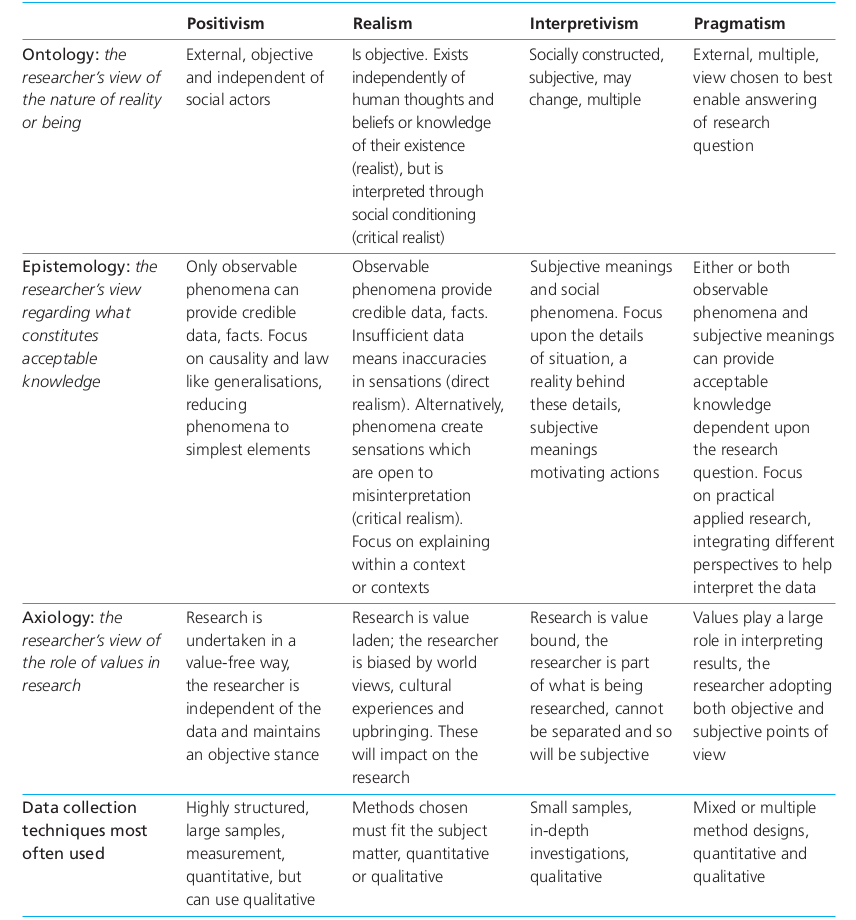
\includegraphics[width=1\linewidth]{img/comparison of research philosophies.png}
    \caption{Comparison of four research philosophies in management research}
    \label{fig:enter-label}
\end{figure}
\par{If the above figure is studied, a separation can be made regarding which research philosophy will be appropriate for the current research study. Positivism immediately stands out because of what its epistemology holds to be true, which is that the only reliable source of information that can be drawn upon is observable phenomena. This suits the current study very well as it will be dealing with a case study to implement a system and the conclusions regarding the success of the development project will be drawn from the success of created artefact or information system. The only other philosophy that has an epistemology aligned to the needs of the research project is realism, as it also views observable phenomena as credible sources of fact, although it opposes a direct reliance on observable phenomena as it believes they can be interpreted incorrectly or with a biased view. Interpretivism and pragmatism regard subjective meaning and social phenomena as the critical source of acceptable knowledge, which does not suit the circumstances of the research project. Therefore, interpretivism and pragmatism are ruled out as options for the chosen research philosophy for this project. }
\par{The remaining two options for viable research philosophies must be compared further to find a suitable methodology for the research project. Within the positivistic approach, the research is taken from a third party point of view to remain objective and reliant on the conclusions drawn from the outcome of the research project, while realism ascertains that the researcher is biased by world views and experiences and that this factors will have an impact on the research. As one of the critical purposes of this research project is to create a replicable methodology for how students can consistently build industry level software solutions, it is of the utmost importance that the researcher remain unbiased and objective. Therefore, according to the comparison of epistemology and axiology between positivism and realism, positivism is chosen as the preferred research philosophy for this project. }
\par{The next section encompasses the following stage within the modified research onion \citep{mardiana2020modifying}, the research approach. This section will be the entry point into the second layer of the research onion.}

\section{Research Approach}
\par{Research approaches make up the second layer of the Research Onion. A research strategy aids in the structure of a study by offering direction in determining the theory that the investigation seeks to advance \citep{saunders2009research}. There are three approaches that are offered by the the modified research, namely deduction, abduction, and induction. These three approaches are each investigated in more depth in the subsections that follow. Once they have been reviewed, a conclusion will be made on which option will be taken forward as the approach for this research project.}
\subsection{Deduction}
\par{In the deductive method, a hypothesis is generated alongside an established theory in order to test the theory \citep{saunders2009research}. When assessing qualitative data, the deductive and inductive approaches offer a thorough method. To make sense of the entire collection of data and comprehend what is taking place, this procedure entails fully immersing oneself in the reading and consumption of the material \citep{azungah2018qualitative}. Deductive qualitative research is distinct from other qualitative methodologies since it utilises conceptual premises generated from the review of literature as its starting point and employs them to the gathering and examination of data\citep{pearse2019illustration}.}
\par{Despite decades of exponential increases in computing capacity, the foundational ideas of the theories of computation still hold true. Thus, the importance of deductive research methods as a source of specific program knowledge has been established over time \citep{eden2007three}. \cite{knuth1968semantics} provides the following justification for his definition of computer science as a sub field of mathematics:}
\begin{quote}
"Like mathematics, computer science will be somewhat different from other sciences in that it deals with man-made laws, which can be [deductively] proved, instead of natural laws which are never known with certainty"
\end{quote}
\par{If the advice of \cite{knuth1968semantics} is taken into consideration alongside the fact that the current research field is computer science, the deductive approach could be very promising to achieving successful results in this project. The next subsection will outline abduction and the potential it holds for being the chosen research approach.}
\subsection{Abduction}
\par{When abduction was first used in 1597 by Julius Pacius to translate the Aristotelian apagoge, it went largely unrecognised for nearly three centuries. The term was initially used by C. S. Peirce \citep{smyth1999peirce}, who stated that it would represent the only fully knowledge-extending method of interpreting that would be categorically different from the two typical forms of logical conclusion, namely deduction and induction. In several artificial intelligence domains, including diagnosis, natural language comprehension, default reasoning, database updates, planning, and high-level vision, this type of abduction has become a common reasoning method.}
\par{Determining the most plausible explanation for a given collection of data is a challenge that can be classified as abduction \citep{josephson1987mechanism}. Abduction is applicable to many different types of reasoning exercises \citep{charniak1985introduction}. For instance, the final diagnosis in medicine clarifies the patient's symptoms and indicators \citep{pople1973mechanization,reggia1983diagnostic}. According to natural language comprehension, a sentence's intended meaning reveals why it was said \citep{hobbs1993interpretation}. Acceptance of a hypothesis in the establishment of scientific theory depends on how well it explains the data. In abductive reasoning, assumption A is accepted if it implies some observation 0 and aligns with preexisting beliefs \citep{lewis1982role}.}
\par{Abduction has become a common reasoning method in various artificial intelligence domains, including diagnosis, natural language comprehension, and planning. In the context of this master's thesis in computer science, abduction offers a systematic approach to evaluating student developers' capabilities and comparing their processes with industry standards, thereby aiding in the creation of an industry-standard ERP system for TaskFlow. Through its emphasis on determining the most plausible explanation for a given collection of data, abduction provides a valuable framework for ensuring the feasibility and success of the research project. As the project progresses, abduction will serve as a guiding principle for identifying and addressing challenges, iteratively improving the system, and ultimately contributing to the advancement of systems development methodologies within both academic and industrial settings.}
\subsection{Induction}
\par{Induction is widely used in the field of computer science (CS). Data structures, philosophy of computing \citep{lynch1996distributed,hopcroft2001introduction,barwise1998computers}, programming languages \citep{pierce2002types}, program efficiency-time complexity \citep{cormen2022introduction}, and algorithm correctness \citep{cormen2022introduction,lynch1996distributed,page2003software,weiss1998data} are only a few of the computer science fields that depend on it. Furthermore, induction can be employed as a teaching strategy to improve students' understanding and performance with CS concepts such as algorithm design, recursion, and programming languages \citep{manber1989introduction,wu1998conceptual}.  According to \cite{bruce2003math}, }
\begin{quote}
        "Programmers with a good understanding of mathematical induction find it much easier to write and, even more importantly, provide convincing arguments for the correctness of recursive algorithms."
\end{quote}
\par{However, research has shown that, even after receiving repeated training in several courses within their curriculum, students typically struggle to comprehend and execute proofs via induction \citep{lowenthal1992mathematical,movshovitz1993mathematical,baker1995characterizing,dubinsky1989teaching}. Even after receiving repeated teaching in several courses within their curriculum, it has been reported in the literature that students generally struggle to comprehend and execute proofs by induction \citep{polycarpou2008conceptual}.}
\par{In conclusion, induction serves as a foundational pillar within the field of computer science, playing a vital role across various domains Its significance extends beyond theoretical frameworks, as it also serves as a pedagogical tool to enhance students' understanding and proficiency in fundamental CS concepts. Despite its ubiquity and importance, empirical evidence suggests persistent challenges among students in grasping and applying inductive reasoning. Addressing these challenges requires a nuanced approach that combines theoretical instruction with practical application, leveraging insights from cognitive science and educational psychology to scaffold students' learning experiences effectively. By acknowledging the complexities inherent in mastering induction, educators and researchers can develop tailored interventions aimed at fostering deeper comprehension and proficiency in this essential aspect of computer science education that could lead to a successful outcome within this research project.}
\par{The research approach that is made use of within this research paper is deduction as it holds that with this approach a researcher begins with a hypothesis and then aims to acquire evidence to prove it, support it, or outrightly refute it. This approach is used by researchers when they want to test an existing hypothesis rigorously. Therefore, it is the most suited to what is being tested in this research project and will further be used as the research approach in this project aiming to make use of the assumption that students can build an ERP system of industry standards and put it to the test. The next section regards the third layer of the modified research onion called the research strategy, where the methods of data acquisition are investigated and the chosen method is then selected.}


\section{Research Strategy}


\section{Research Methodologies}
%What is a research methodology and what is its purpose? WRITE INTRODUCTION
\subsection{Design Science}
\par{The Design Science Research Methodology, or DSRM, was developed by \cite{peffers2007design} with three goals in keeping in mind: "(1) offer a nominal procedure for carrying out DS study, (2) expand on earlier research on DS in IS and related fields, and (3) offer scholars a conceptual model for a framework for the results of research.” The Design Science Research (DSR) paradigm is based on the artificial sciences and engineering. In essence, it is a paradigm for solving problems. DSR creates new artefacts in an attempt to advance human understanding \citep{hevner2010design}. In the past few years, a number of researchers have successfully brought design research into the realm of information science (IS) studies, such as \cite{hevner2004design} and \cite{walls1992building}. They are also effective in making design a major part of research and proving the value and legitimacy of design science (DS) as an IS research paradigm. In the fifteen years or more that have elapsed since those first articles, very little DS research has been successfully published in the IS field, despite these effective breaches \citep{peffers2007design} outlines a process that encompasses six activities that make up the DSR methodology and are arranged in a certain sequence that dictates the order of progression for research based on this methodology. The table below outlines these activities.:}
\clearpage
\begin{figure}[h!]
    \centering
    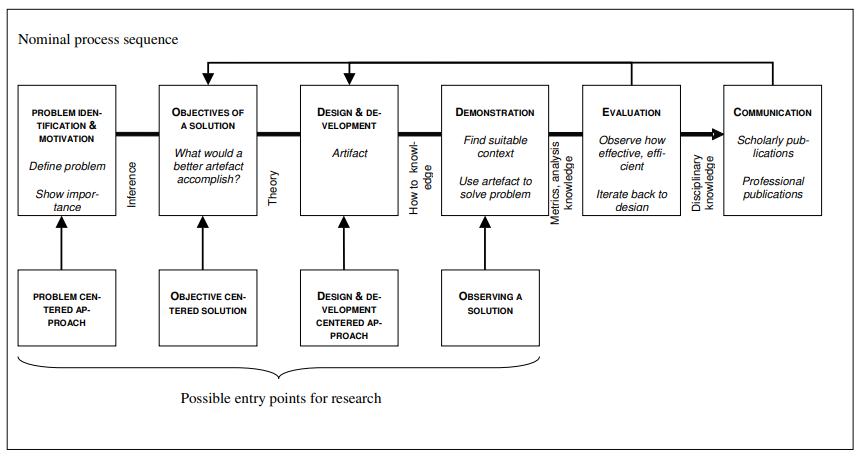
\includegraphics[width=1\linewidth]{img/Design science research process (DSRP) model.png}
    \caption{Design science research process (DSRP) model}
    \label{fig:enter-label}
\end{figure}
\par{The DSR methodology will be used to conduct the research project, thus each step outlined by \cite{peffers2007design} is investigated in broader context to better understand accurate execution and use of the research methodology.}
\par{\begin{enumerate}
        \item Problem Identification and Motivation
\par{Before coming up with viable solutions, designers work with vague problems that need more investigation (\citealt{buchanan1992wicked, rittel1973dilemmas}). Prescriptive engineering design procedures frequently place a strong emphasis on characterising an issue as the first step. Problem  is the driving force behind these problem-first approaches, which use design to find a solution \citep{dewey2022we}. There for it is of the utmost importance to correctly identify and define the problems and motivation within this research study.}
\par{The purpose of this first activity within the research methodology is of utmost importance as it designates the entry point to the entirety of what will be done within this research. \cite{peffers2007design} specifies what has to be done to properly identify the problem and motivation related to the study. The research problem has to be specified and an explanation to why a solution is valuable must be provided. It could be helpful to conceptually atomize the problem so that the solution can adequately represent the complexity of the problem, as the problem definition will be utilised to create an effective artifactual solution. Two goals are achieved when a solution is justified: first, it encourages the researcher and the research's audience to pursue the answer and accept the findings; second, it clarifies the logic behind the researcher's comprehension of the issue. Knowledge of the problem's current condition and the significance of its solution are among the resources needed for this task.}
        \item Objectives of the solution
\par{Determine a solution's goals based on the definition of the problem. The goals can be qualitative, such as when a new artefact is anticipated to enable answers to issues not previously addressed, or quantitative, such as terms in which a desirable solution would be preferable to current ones. The goals ought to be as follows: logically inferred from the problem description. Information about the current state of issues, existing solutions, and their efficacy, if any, are among the resources needed for this.}
        \item Design and Development
\par{}
        \item Demonstration
        \item Evaluation
        \item Communication
\end{enumerate}}
\subsection{Action Design Research}
\subsection{Action Research}
\subsection{Conclusion}


\section{Research Design}
A researcher's detailed approach for addressing his or her research question(s) is known as the research design \citep{mardiana2020modifying}.
\subsection{Data Collection}
\subsection{Ethical Considerations}


\section{Conclusion}

\chapter{Literature Study}
\par{Enterprise Resource Planning (ERP) systems have become a cornerstone in the modern business
landscape, facilitating the integration and management of various organizational processes. 
These systems, characterized by their comprehensive features and functionalities, are designed 
to streamline operations, enhance efficiency, and provide real-time insights. This literature 
review explores the multifaceted nature of ERP systems, delving into their features, the 
competitive dynamics within the ERP industry, and the essential components that define an 
industry-approved software system.

The subsequent sections address the broader context of the information technology industry, 
highlighting the challenges it faces globally and within developing nations specifically. The role 
of universities in bridging the gap between academic knowledge and industry requirements is 
examined, with a comparative analysis of the unique challenges faced by developing nations versus 
more developed regions.

A thorough examination of the value chain in software development is provided, focusing on 
the critical aspects of people, processes, technology, hardware, software, and infrastructure. 
This section also considers the economic viability of partnerships between academia and industry, 
emphasizing the mutual benefits and resource-sharing opportunities.

The review further investigates the commercialization of software, discussing various methods 
and offering recommendations for effective commercialization strategies. The role of students in the
industry is explored, considering the advantages, potential threats, and comparisons with similar 
projects undertaken elsewhere. An in-depth analysis of project management methodologies relevant to software development is presented, along with specific recommendations tailored to the context of ERP systems. Implementation frameworks are examined to identify critical competencies required for successful 
software development, followed by targeted recommendations. Finally, the review discusses the artefact of ERP systems, presenting methods for measuring the success and functionality of such systems. The Technology Acceptance Model (TAM) is utilized as a framework to evaluate user acceptance and effectiveness.

This comprehensive literature review aims to provide a detailed understanding of the 
complexities involved in students building ERP systems for industry, offering insights into best 
practices, challenges, and strategic approaches for successful implementation and commercialization.}

\section{ERP Systems}
\par{The ERP archive, which dates back to possibly 1970, was started with the intention of integrating business activities \citep{shields2004business}. Material Requirement Planning (MRP) systems, which were created in the 1960s and 1970s and allowed manufacturing to be planned according to projected demand rather than past information for the first time, are the ancestors of Enterprise Resource Planning (ERP) systems \citep{ahlawat2017role}. ERP delivers real-time data from a single centralised database and is multidisciplinary, multipurpose, and multidimensional, in contrast to MRP, which was restricted to procurement, production, and manufacturing. It links and unifies every department across the whole company. The various vendors—known as best of breed implementations—such as those from the designated "big five"—SAP, Oracle, PeopleSoft, JDE, and Baan—which together account for around 70 percent of the ERP market—can be used in tandem with one another \citep{light2001erp}. 

ERP was first used at the beginning of 1990, and it was named by the Gartner Group \citep{chang2000delphi}. The early 1990s saw the introduction of ERP by software companies like SAP. In 1992, SAP released the R/3 version once more. Customer-server hardware structure was added to the SAP R/3 so that it could operate on many stages at once \citep{jacobs2007enterprise}. By 2000, all the main ERP software system providers had solved the Y2K challenge. By connecting business and management activities, enterprise resource planning (ERP) tools assist organisations in realising their full potential \citep{uccakturk2013effects}. Business patterns will shift over the next ten years as a result of modifications to a vertical market, application techniques, and the ERP cost structure. Cloud application models are stored in a lot of data. SaaS, for instance, is attracting businesses' attention. Business enterprises seeking to reduce significant capital costs through a monthly subscription model have embraced the ERP pricing model, which charges based on usage \citep{kenge2020research}.

\cite{zhao2021research} propose a generalised architecture for the functional design of an ERP system that can be very helpful in understanding the purpose of these systems and what they do. The diagram that describes this functional architecture can be seen below:}
\linebreak
\begin{figure}[ht!]
    \centering
    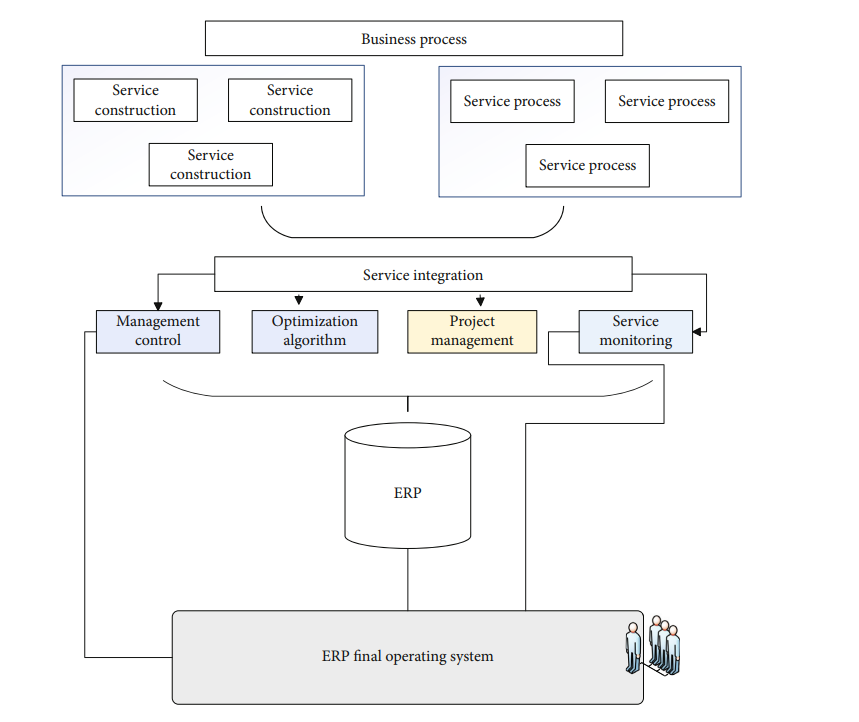
\includegraphics[width=1\linewidth]{img/ERP system framework hierachy.png}
    \caption{ERP System Framework Hierarchy}
    \label{fig:enter-label}
\end{figure}
\par{The diagram shows how an ERP system interprets the defined business process and how it processes this information to generate an effective output. The services that occur during the business process are integrated with a system that monitors, optimizes, and manages these processes and in turn a completed ERP system is created. }
\subsection{Features of ERP Systems}
\par{There are various features that make up an ERP system, however there is no set standard for what an ERP system must be able to functionally do as ERP systems are configured for the need of the company it is built for. However, generally ERP systems can potentially have any of the following features that are discussed and examined below:}
\subsubsection{Financial Management}
\par{The benefits of implementing enterprise systems for accounting have not been thoroughly studied globally. Furthermore, there are surprisingly few studies that thoroughly investigate the connection between ERP user happiness and accounting gains \citep{kanellou2013accounting}. Nonetheless, there are studies concentrating on the relationship involving ERP systems and accounting in the pertinent literature. \cite{spathis2004enterprise} investigated the adjustments taking place in terms of accounting software as well as the factors that led businesses to decide to replace their outdated information systems with fully functional ERP systems. The findings demonstrated that the three primary drivers of ERP adoption were the growing requirement for immediate data, the requirement for integration between applications, and the production of information for decision-making. Greater data production flexibility, increased accounting application integration, better report quality (statement of accounts), better decision-making based on timely and accurate accounting information, and a shorter yearly account closure period were the main accounting benefits of ERP implementation.

It was discovered that ERP systems can support novel accounting procedures and serve as data sources for them. More precisely, ERP systems appear to help with data collecting and the organisational scope of management accounting, according to \cite{rom2006enterprise} This was further supported by \cite{spathis2004enterprise} who pointed out that the use of these systems encourages the adoption of innovative management accounting practices and improves accountants' efficiency in carrying out daily tasks, managing large databases, and producing reports swiftly and adaptably.

\cite{kanellou2013accounting} concluded that there are several advantages to using an ERP in the accounting department, and the most of these are well regarded. Therefore, the case can be made that an organisation should integrate accounting with its ERP system. Lastly, it is noted that there is a positive correlation between ERP cost and ERP advantages and the degree of ERP user satisfaction. These conclusions are very encouraging and as financial management is a lacking feature within the TaskFlow system, the further development of this integral functionality will be made a priority throughout the case study project.}
\subsubsection{Human Resources Management}
\par{Enterprise managers' main concerns in modern times are increasingly intense business competition amongst enterprises and how to draw in the best talent to become part of the workforce, streamline human resources, cut personnel costs, and increase the competitiveness of enterprises; in other words, these enterprise managers believe that the integration of ERP into the HR system has expanded the system's capabilities to encompass enterprise management. The variety of HR services has expanded as well, from payroll accounting and personnel administration to a comprehensive suite of tools that support business decision-making. Planning for human resources, staff appraisal, scheduling, time management, hiring, payroll, training initiatives, and travel administration are some of these topics. They combine to create an effective and highly integrated ERP, together with the financial and production systems \citep{zhao2021research}.

\cite{zhao2021research} proposes a figure showing the impact of ERP systems in increasing the efficiency of HR procedures within a business. The figure can be seen below and proves the worth and effectiveness of implementing this type of system into the HR workforce.}
\begin{figure}[ht!]
    \centering
    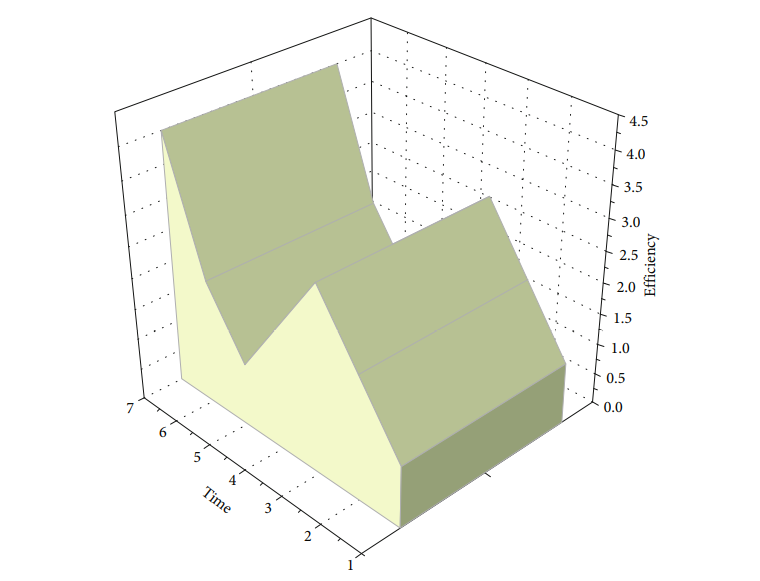
\includegraphics[width=1\linewidth]{img/Human resource management system optimization rate..png}
    \caption{Human resource management system optimization rate}
    \label{fig:enter-label}
\end{figure}
\subsubsection{Supply Chain Management}
\par{The ERP's supply chain component manages all retail operations, including shipments, receipts, issues, and quality control. If you work for a manufacturer, wholesaler, or retailer, managing your inventory is essential to keeping expenses under control and guaranteeing the seamless running of your company. The core functions of every organisation, stock management and valuation, require a significant investment of time and money. Every item's lot-by-lot stock is kept track of, and several computerised information reports are offered to monitor stock movement \citep{ahlawat2017role}.

The ERP supply chain activities include determining the amount of inventory needed, establishing goals, receiving and delivering goods, maintaining materials in stock subsections, categorising every product, supplying materials to the fabrication department, and fully documenting supplier rejections. Additionally, it offers alternatives and strategies for restocking, keeps track of item usage, reconciles inventory balances, and reports the state of inventory \citep{ahlawat2017role}.}
\subsubsection{Customer Relationship Management (CRM)}
\par{The phrase "customer relationship management (CRM)" refers to the capacity to continuously engage with customers across a range of channels; it offers the frameworks necessary for businesses to grow and improve their customer offerings and draw in new ones. Companies are now more interested in knowing their customers and interacting with them in order to seize opportunities and overcome obstacles as a result of the growing rivalry in the business world \citep{kostojohn2011crm}.

Early in the 1990s, CRM was created with the purpose of managing sales teams and direct marketing, as well as preserving consumer data and reaching their preferences from past purchases and conversations \citep{bygstad2013social}. CRM was created to provide a range of essential tools that could be used by businesses of all sizes and in a variety of industries. These tools would enable them to monitor, manage, and share customer data \citep{smilansky2015select}, aid salespeople and marketers in examining the behaviour of their clients, and add value to the company through the use of both human and technological resources \citep{bibiano2014initial}. Therefore, businesses become more competitive, maximise revenues, decrease effort duplication, improve the effectiveness of information storage, make it available to all employees, and provide a single overview to partners and customers. CRM systems comprise the techniques, tools, and capacities that assist an organisation in managing its customer relationship. A significant portion of this work is closely related to the advancement of information and communication technology, which allows businesses to gather the most data possible about their clients' behaviour, contact details, and other characteristics. It also gives them access to efficient tools and methods for managing this data. Thus, the concept of CRM refers to the ability for businesses to better manage their clientele by implementing dependable systems, processes, and procedures that enable them to obtain the most data about their clientele and interact with them for business objectives in order to obtain specific information that aids in the targeting of goods, services, and new markets \citep{ronchi2009eculture}.}
\subsubsection{Inventory Management}
\par{Real-time data on inventory levels and values, encompassing stock on order, raw materials, ongoing work, and completed products, is provided by ERP software. The ERP inventory component handles all aspect of a company's stock-related operations. An inventory management module is a tool that makes collecting information in the inventory department or warehouse quicker and can assist you in keeping the right amount of stock on hand \citep{ahlawat2017role}.

The supply and demand sides benefit from the application of an inventory management methodology. Inventory management can improve the speed of delivery and stabilise interactions with clients for the supply side. On the demand side, it also lessens the impact of inventory on financial resources, lowers the possibility of material deficits, and quickens the supply chain's reaction time \citep{zhao2021research}.

\cite{zhao2021research} proposes two a flow charts that symbolise the functioning of production, inventory, procurement, and the payment process within an ERP system. This example can be further generalised and seen as a general flow chart of how and ERP system technically and practically functions within a given component of the system which in this case is inventory management. Both these flow charts can be studied below:}
\begin{figure}[ht!]
    \centering
    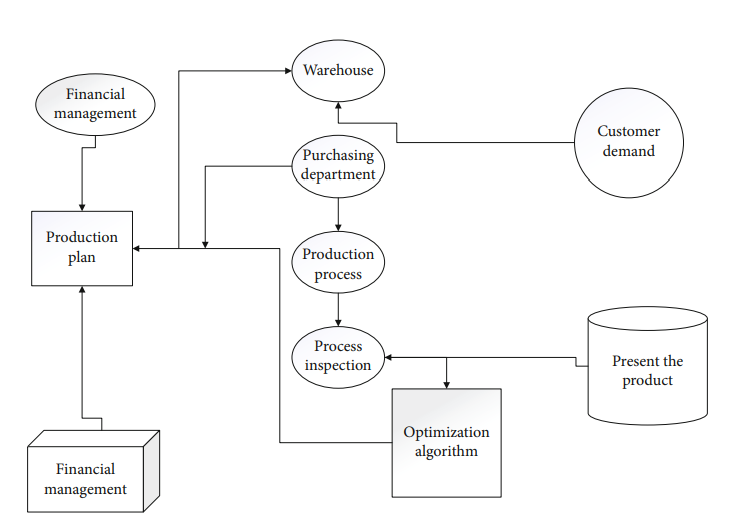
\includegraphics[width=1\linewidth]{img/rename flow chart of company's inventory and production.png}
    \caption{Flow chart of the company’s production and inventory business based on ERP system}
    \label{fig:enter-label}
\end{figure}
\pagebreak
\begin{figure}[ht!]
    \centering
    \includegraphics[width=1\linewidth]{img/Flow chart of the company’s ERP-based procurement and payment process.png}
    \caption{Flow chart of the company’s ERP-based procurement and payment process}
    \label{fig:enter-label}
\end{figure}
\par{Within this basic examples we can see how the business process would hypothetically flow and how data moves to and from a database storing the information necessary to produce some sort of return. This concept can be applied throughout various modules of an ERP system. Each function is always user input that is processed, stored in a database, and then an output that is once again returned to the user.}
\subsubsection{Sales and Marketing}
\par{A system was created as a tool to address particular business functions beginning in 1975 \citep{monk2013concepts}. This technology allows for the automation of business function-related tasks and transactions. Nevertheless, the organization's inter-area business operations must manually transfer data because each system is tailored to a particular business function and there is no system integration. Therefore, the likelihood of data duplication is relatively high. For instance, if the finance and supply chain functions also need data on the sales business function, the data is just being reproduced to meet the requirements. This is the primary justification for using a single database for incorporating part or all of an organization's business processes through enterprise resource planning.

It is anticipated that this technology will enable all organisational transactions to be automated and eliminate the requirement for manual data sharing amongst all business operations. Because of this, having an ERP system in place is crucial to an organization's ability to operate profitably \citep{tsai2008impact}.
    
A business is a company that makes money by selling products or services to customers. Many of the transactions that take place throughout its operation involve businesspeople. The transactions typically comprise a range of organisational data, such as the quantity of inventory, the volume of revenue flowing in and going out, the quantity of goods that need to be produced. Furthermore, transactions typically result in the production of a number of documents, including sales orders, invoices, quotes, and inquiries \citep{xu2008review}.

By making proper use of an ERP system to automate and manage sales and marketing tasks, \cite{terminanto2017implementation} suggests the following improvements can be made:}
\begin{itemize}
    \item Employ an ERP system to save and combine data from all divisions into a single system.
    It is anticipated that divisions will be able to coordinate more effectively with the data recorded in the system.
    \item Generating a quote form through the ERP system. Sales no longer have to access different kinds of papers in order to finish filling out the offer form thanks to the ERP system. Sales can access the system's database and enter the information required to create a quote straight away. Additionally, since the quotation form is automatically prepared and kept in the system, sales do not need to save it in and external system.
\end{itemize}
\subsubsection{Business Intelligence (BI)}
\par{Business Intelligence (BI) solutions are becoming the centre of attention for companies when it comes to information systems. The advantages of business intelligence (BI) differ greatly amongst companies. Due to their ability to combine, integrate, and analyse the massive volumes of transactional data produced by ERP systems, business intelligence (BI) solutions are increasingly utilised as extensions of ERP systems \citep{hawking2010business}.

New apps and the growth of current IT systems were brought about by the need for better information analysis as well as advancements in related technologies.
Collaborative systems (CS), corporate performance management (CPM), analytics, knowledge discovery (KD), data mining (DM), and knowledge management (KM) were among them. All of the above listed systems are now frequently referred to as business intelligence (BI) \citep{gibson2004evaluating,olszak2007approach}.

In today's corporate environment, business intelligence (BI) is deemed highly priority by many firms due to its potential to significantly impact their performance. Companies who employ business intelligence (BI) properly can generate an average return on investment (ROI) of 401 percent over a three-year period, according to \cite{power1998justifying}. 70 percent of the 142 organisations surveyed by \cite{herzum2003cutter} reported that they were putting data warehousing and business intelligence efforts into practice. Leading business analyst firm \cite{gartner2009gartner} polled 1,500 Chief Information Officers globally and determined that business intelligence (BI) was the most important technology priority. Accordingly, it is predicted that by 2012, revenue from BI vendors will amount to 7.7 billion dollars \citep{sommer2008gartner}.}
\subsection{Competition within the ERP System Industry}
\par{The biggest players within the ERP space are SAP, Oracle, and Microsoft. These companies provide the software solutions for business process management on the largest scale. These companies are direct competitors for one another but have less impact on small and medium sized companies who rather go for more affordable and practical solutions. Within the South African space, these small and medium companies make use of Monday.com, Zoho, SalesForce, Clickup, and similar software such as what is being built and sold at Taskflow. This section will proceed to review and compare these various providers and their commercialised systems to determine what commonality there is between them and identify the base requirements of a fully functional ERP system.}
\subsubsection{SAP}
\par{In 1972, Hopp, Wellenreuther, Hector, Plattner, and Tschira developed the SAP method \citep{o2015sap}. The SAP method is made up of a number of fully integrated components that cover almost every aspect of a professional organisation. The SAP approach is the primary source of supply for the ERP system keys industry. In 2012, the SAP software system held around 25 percent of the market and industry.However, Oracle software came in second with 13 percent of the market share, followed by Microsoft Dynamics with 5 percent. SAP is a very large company that does not focus exclusively on its most lucrative ventures. Their produce is truly minor commercially approachable, catering to hundreds of customers who make up less than 1,000 society members. 

When one learns the fundamentals of the SAP software system, it becomes a simple tool to utilise even though it may take some time for individuals unfamiliar with it to make the switch from Microsoft Dynamics and Oracle. SAP software systems tend to be more expensive than their competitors, even though prices can vary depending on features and benefits. This makes them less than ideal for small to medium-sized businesses with limited IT funding \citep{annamalai2011enterprise}.}
\subsubsection{Oracle}
\par{Oracle software E-Business Collection \citep{barr2014oracle} is a potent ERP programme with a wide range of features and advantages that have helped elevate it to the status of one of the most advanced ERP programmes available today. For ease of use, Oracle software system E-Business Group may smoothly merge several components into a single system. Additionally, Oracle E-Business Group enables users to automate a number of processes, eliminating the need for human data entry. In addition to increasing efficiency and productivity, this also fixes errors and guarantees that data is not lost. 

The Oracle software system E-Business Collection has the ability to record the course of inventory levels at Business Company. Should an item's inventory level drop beneath a predetermined positive standard, the system will immediately provide purchase orders. Very powerful, durable, and intuitive ERP software is the Oracle software system EBusiness Collection, which can meet the needs of almost any industry. Businesses build their own individual elements since the predefined tax element and sales units on the Oracle E-Business Group are frequently insufficient \citep{barr2014oracle}.}
\subsubsection{Microsoft}
\par{Microsoft Dynamics Marketing is built on Microsoft infrastructure, as its name implies. It synchronises and develops flawlessly with additional Windows commercial requests, facilitating the effortless distribution of data across all methods organisations. Microsoft Dynamics synchronises with various Windows applications, as previously mentioned, simplifying data sharing and transfer. It is built on a Windows substructure and takes a lot less time to implement Microsoft Dynamics Marketing than other approaches. takes the least amount of time to apply out of the three, according to Panorama Consulting Solutions \citep{solutions2016report}. Large, international industries find Microsoft Dynamics ideal as it supports multiple languages and can work with a variety of currencies in close proximity to global marketing.}
\par{\cite{mayer2017clash} proposes the table below to draw comparisons between these three ERP systems:}
\begin{table}[ht]
    \centering
    \scriptsize
    \begin{tabular}{|l|c|c|c|}
    \hline
    & \textbf{SAP} & \textbf{Oracle} & \textbf{Microsoft Dynamics} \\ \hline
    Store Part & 19\% & 13\% & 16\% \\ \hline
    Short-list Rate & 38\% & 18\% & 31\% \\ \hline
    Collection Rate When Short Recorded & 38\% & 22\% & 22\% \\ \hline
    Application Period & 23.1 months & 24.5 months & 23.6 months \\ \hline
    Total Price of Ownership & \$2.09 million & \$2.38 million & \$2.06 million \\ \hline
    Reimbursement Period & 30 months & 29 months & 12 months \\ \hline
    Disruption at Go-live & 44\% & 42\% & 41\% \\ \hline
    Realised 50\%+ of Anticipated Business Benefits & 34\% & 21\% & 26\% \\ \hline
    \end{tabular}
    \caption{Comparison of SAP vs. Oracle vs. Microsoft Dynamics}
\end{table}
\par{The table shows that all three of these systems perform similarly across the measurement categories, however it seems SAP remains the most popular and sits in the middle of the three systems when it comes down to cost of ownership and is the most successful in terms of realising the anticipated benefits of system implementation.}
\subsubsection{Monday.com, Zoho, and Taskflow}
\par{These are the three relevant systems when it comes to the ERP system in South Africa. While there are other competitors such as ClickUp, not all available systems will be reviewed in this research paper as there are large amounts of ERP systems available and the lines between what is classified as ERP and what is not have become blurred, therefore it is only necessary to review these three systems. As SAP, Oracle, and Microsoft have overpowered the industry in terms of landing large corporations as clients, these three systems and many others aim to fulfill the needs of small and medium-sized businesses. In this subsection the function of these three systems will be outlined and then compared to review the differences.

Monday.com is a cloud-based work operating system that enables groups to design workflow applications for managing daily tasks, projects, and procedures. For organising, monitoring, and controlling tasks and projects, it offers a versatile and graphical platform. Customisable workflows, task management, team collaboration tools, and interfaces with several third-party apps are some key features. By providing communication, file sharing, and reporting capabilities in one location, it is intended to increase efficiency and simplify project administration \citep{monday.com}.

Zoho is a comprehensive suite of cloud-based business applications designed to help organisations manage various aspects of their operations. It includes tools for customer relationship management (CRM), finance, human resources, project management, email, and collaboration. Zoho's products are known for their integration capabilities, allowing businesses to streamline processes and improve efficiency. The platform is widely used by small to medium-sized enterprises for its affordability, scalability, and extensive range of features \citep{zoho}.

Taskflow is a software platform designed to manage and automate workflows and tasks within an organisation. It provides tools for task management, project tracking, and process automation, enabling teams to collaborate efficiently and stay organised. Taskflow typically includes features like customisable workflows, task assignments, deadline tracking, and reporting. It is designed to adapt to various business needs, helping improve productivity and streamline operations by ensuring that tasks are completed in a structured and timely manner \citep{taskflow}. The table below compares these various systems.}
\begin{table}[h!]
    \centering
    \resizebox{\textwidth}{!}{
    \begin{tabular}{|l|l|l|l|}
    \hline
    \textbf{System} & \textbf{Monday.com} & \textbf{Zoho} & \textbf{TaskFlow} \\ 
    \hline
    \textbf{Core Functionality} & 
    \begin{tabular}{l}
    - Task and project management \\
    - Customisable workflows \\
    - Team collaboration tools \\
    - Integrations with third-party apps
    \end{tabular} & 
    \begin{tabular}{l}
    - Customer relationship management (CRM) \\
    - Finance management \\
    - Human resources \\
    - Project management \\
    - Email and collaboration tools
    \end{tabular} & 
    \begin{tabular}{l}
    - Task management \\
    - Project tracking \\
    - Process automation \\
    - Customisable workflows \\
    - Reporting
    \end{tabular} \\
    \hline
    \textbf{Pricing} & 
    \begin{tabular}{l}
    - Varies based on plan: Basic, Standard, Pro, Enterprise \\
    - Starting at around \$8/user/month
    \end{tabular} & 
    \begin{tabular}{l}
    - Varies widely depending on products chosen \\
    - Free and paid tiers \\
    - Zoho One: \$37/user/month for the full suite
    \end{tabular} & 
    \begin{tabular}{l}
    - Custom pricing based on business needs \\
    - Typically enterprise-level pricing
    \end{tabular} \\
    \hline
    \textbf{Attributes} & 
    \begin{tabular}{l}
    - Visual and user-friendly interface \\
    - Highly Customisable \\
    - Suitable for teams of all sizes \\
    - Strong integration ecosystem
    \end{tabular} & 
    \begin{tabular}{l}
    - Comprehensive suite of business applications \\
    - Scalable for small to medium-sized businesses \\
    - Strong focus on affordability and integration \\
    - Extensive range of features
    \end{tabular} & 
    \begin{tabular}{l}
    - Designed for workflow automation \\
    - Adaptable to various business needs \\
    - Focused on improving productivity and task management \\
    - Enterprise-level customization and support
    \end{tabular} \\
    \hline
    \end{tabular}
    }
    \caption{Comparison of Monday.com, Zoho, and Taskflow}
\end{table}
\par{The data in the table displays that these systems catering more towards small and medium sized businesses have each found their own business model and sales strategy to increase engagement in their target market as each of these three systems cater for a different audience and have different core functionality.}
\subsection{Components of Developing an Industry Approved Software System}
\par{This subsection and the one that follows will both review the process of creating and implementing an industry approved software system as well as an industry approved ERP system. These subsections will review the standard components of an industry systems development lifecycle and will make reference to the standards and practices that need to be upheld in order for these systems to be successful within the climate of the software development industry, not only in the South Africa, but also the rest of the world.}
\subsubsection{Requirements}
\par{Gathering, examining, and recording stakeholder demands and limitations is the process of requirements analysis, which makes sure the software system satisfies their needs \citep{doe2011recommended}. Since it establishes the framework for all upcoming development efforts, this stage is crucial. Both functional and non-functional requirements—which specify how the system should operate, such as scalability and reliability—should be included in effective requirements documentation \citep{sommerville2011software}.}
\subsubsection{Systems Design}
\par{A blueprint for building the software system is created by system designers using requirements. Determining the \citep{jacobson2021unified}. Good design makes sure that the system's structure satisfies its needs and is efficient, scalable, and maintainable.}
\subsubsection{Implementation}
\par{Developing the program in accordance with the design standards is part of implementation. During this stage, code is written, reviewed, and integrated to make sure it complies with quality standards and design criteria. Maintaining code quality requires adhering to best practices in coding, which include employing version control and coding standards \cite{mcconnell2004code}.}
\subsubsection{Testing}
\par{Testing confirms that the programme satisfies all requirements and functions as planned. It includes a variety of testing techniques, including system testing (evaluating the complete system), integration testing (examining how components interact), and unit testing (evaluating individual elements) \citep{istqb2011foundation}. Finding and fixing issues before release is the main objective \citep{myers2011art}.}
\subsubsection{Quality Assurance}
\par{Planned actions are taken as part of quality assurance (QA) to guarantee that software fulfils quality standards at every stage of development \citep{team2002capability}. This include creating quality measures, carrying out evaluations, and putting procedures in place to raise the standard of quality. QA seeks to stop errors and guarantee dependable and effective software \citep{international2011systems}.}
\subsubsection{Deployment}
\par{Software must be released into the production environment in order for deployment to take place. This stage involves setting up the program, installing it, and making sure it runs properly in a live environment. Thorough preparation is necessary for a successful deployment in order to reduce disruptions and guarantee a seamless transition for users \citep{sommerville2011software}.}
\subsubsection{Maintenance}
\par{Software systems need to be updated and fixed on a regular basis after they are deployed. To guarantee that the program continues to satisfy the requirements of users and runs safely and effectively, maintenance entails correcting, adaptive, and preventative actions \citep{pressman2005software}. An essential component of the maintenance stage is managing patches and version updates.}
\subsubsection{Security}
\par{To protect the system from weaknesses, security is incorporated across the whole lifetime. According to \cite{goodrich2011introduction}, these include of restricted access, the use of encryption, secure programming techniques, and frequent inspections of security. To make sure the infrastructure is resistant to threats, penetration tests and vulnerability inspection are helpful.}
\subsubsection{Documentation}
\par{Regarding both current development and upcoming upgrades, comprehensive documentation is crucial. This includes system architecture, code, user manuals, and maintenance procedures \citep{doe2011recommended}. By acting as a communication mechanism between stakeholders, documentation guarantees the maintainability and understandability of the system.}
\subsubsection{Compliance}
\par{According to \cite{sommerville2011software}, compliance is the system's conformity to legal, regulatory, and industry standards including SOX, GDPR, and HIPAA. Compliance guarantees that the system complies with legal requirements for data security, privacy, and operational openness.}
\subsection{Components of Developing an Industry Approved ERP System}
\par{This subsection will once again review the same components as before, except making specific reference to ERP systems, how they differ from other system implementation within the software industry, and providing detail into actions within the process that result in a successful systems development process.}
\subsubsection{Requirements}
\par{Due to the cross-functional nature of ERP systems—which integrate numerous business processes—gathering requirements is one of the most important stages of the process. ERP systems must take into account the needs of different divisions, notably supply chain, customer relationship management (CRM), finance, and human resources, as opposed to normal software projects. ERP failure can result from incorrect or poorly stated requirements, which is concerning considering the high expense and complexity associated with ERP implementations \citep{monk2013concepts}. The requirements gathering process, which makes sure the ERP system will fulfil organisational goals, consists of several steps, including discovery, stakeholder interviews, and business process modelling \citep{esteves2001enterprise}. }
\subsubsection{Systems Design}
\par{According to \cite{monk2013concepts}, ERP systems are made to be modular, enabling businesses to implement just the elements they need to run the system without compromising its integrity. While one module must fluidly interface with the others, system design is made more complex by this modularity. The financial module of an ERP system, for instance, needs to interface with the modules for inventory, procurement, and manufacturing in order to guarantee correct financial reporting. Scalability is another important consideration in system design because enterprise environments typically have high transaction and user volumes \citep{o2000enterprise}. The ERP software that is selected has a significant impact on the design phase. Programs like SAP, Oracle ERP, or Microsoft Dynamics have predefined workflows and data structures that need to be customised to meet the unique requirements of the company. The incorporation of external systems, such as customer relationship management (CRM) software and business intelligence (BI) platforms, should also be taken into account throughout the design phase as it is common practice create intergrations between different platforms due to client requirements.}
\subsubsection{Implementation}
\par{The process of implementing an ERP involves several stages, including configuration, training, data migration, and customisation. According to \cite{zhang2003critical}, customisation usually refers to changing ERP modules to satisfy certain business demands, including special processes or regulatory constraints. Contrarily, configuration entails adjusting the ERP system's parameters—like tax rates or payment terms—to match the operational framework of the company. Data migration, or moving data from old systems into the ERP, is one of the trickiest parts of implementing an ERP. Due to data inconsistencies, missing data, or variations in data architecture, this might get complicated. To reduce disruption, ERP systems usually take a staged approach, rolling out modules one at a time \citep{shanks2000model}. }
\subsubsection{Testing}
\par{According to \cite{ahmad2013critical}, testing in ERP systems is more complicated than testing in traditional software since ERP connects several business processes from different departments. Integration testing examines the interactions between these modules, whereas functional testing verifies that each module—for example, finance, HR, and procurement—functions as intended. For instance, adjustments to inventory levels ought to be automatically reflected in the finance module. Because it involves end users running real-world scenarios, user acceptability testing (UAT) is essential to verifying that the system satisfies business needs \citep{nah2001critical}. Furthermore, especially in international organisations, performance testing is essential to guarantee that the system can manage large numbers of users and transactions. To safeguard critical data, like payroll data and financial records, ERP testing should also involve security testing.}
\subsubsection{Quality Assurance}
\par{ERP systems use quality assurance (QA) to make sure the solution satisfies technical and business objectives and is error-free \citep{hawari2010explaining}. QA is a multi-layered process that begins with automated testing and code reviews to identify problems early in the development cycle. Validating that business processes match the ERP configuration and that workflows and transactions flow correctly between modules is another aspect of quality assurance (QA) in ERP installations. Due to the significant financial and operational risks connected with defects—which could lead to erroneous financial reporting, disruptions in the supply chain, or non-compliance with regulations—quality assurance (QA) is crucial for ERP systems \citep{hawking2004revisiting}. ERP providers frequently offer QA-specific solutions, like SAP's Solution Manager, which aids businesses in managing their QA procedures.}
\subsubsection{Deployment}
\par{ERP deployment is usually carried out in stages to reduce business impact. This usually entails introducing one department or module at a time, beginning with less important tasks and working your way up to more crucial ones like supply chain management or finance \citep{monk2013concepts}. While more risky, "big bang" deployment strategies—where the entire system goes online at once—are occasionally chosen by businesses that need to make urgent system-wide modifications. Because they provide more flexibility, quicker deployment periods, and lower infrastructure costs than conventional on-premise systems, cloud-based ERP systems—like Oracle ERP Cloud or SAP S/4HANA Cloud—are becoming more and more popular \citep{vukovic2023erp}. Cloud-based ERP systems, however, could run into issues with data security, compliance, and limited customisation options.}
\subsubsection{Maintenance}
\par{After going online, maintaining the ERP system becomes a constant effort that involves routine upgrades, bug patches, performance enhancements, and modifications to accommodate evolving corporate needs \citep{ahmad2013critical}. Patches and upgrades are routinely released by ERP suppliers; these must be tested and implemented without interfering with regular business operations. Updating the system to account for new business procedures or regulatory changes—like entering new markets—is another aspect of maintenance. Maintaining ERP effectiveness is essential to keeping the system in line with the changing needs of the company. Reduced ROI, elevated security threats, and operational inefficiencies might result from improper ERP system maintenance \citep{hawking2004revisiting}.}
\subsubsection{Security}
\par{ERP systems manage enormous volumes of sensitive data, including personnel records and financial data, thus security is a top priority. Access controls, encryption, and frequent audits are only a few of the layers that make up ERP system security \citep{tarafdar2003analyzing}. ERP systems frequently employ role-based access control (RBAC) to make sure that users can only access information and take actions that are appropriate for their position. ERP providers help businesses manage risks and maintain regulatory compliance by offering integrated security capabilities, such as SAP's Governance, Risk, and Compliance (GRC) solutions \citep{hawari2010explaining}. To find possible threats and reduce risks, regular penetration tests and vulnerability assessments are crucial.}

\section{Implementation of ERP Systems}
\par{The seven main steps in the ERP deployment process include business process analysis, software installation, data migration, software performance testing, user training, complete deployment, and post-implementation support \citep{ly2020definitive}. These main key steps are examined in greater depth in the sections that follow.}
\subsubsection{Software Installation}
\par{Following the first step's creation of new procedure flows, the team should have a new business process plan in place. The architecture and infrastructure for software, such as the data store, data presentation, and internet accessibility, will be installed and constructed by the software developers who have recieved the business requirements from the business analyst.}
\subsubsection{Data Migration}
\par{In this stage, all data is transferred to a new software platform. Before the data is transferred to a new site, it should all be reviewed and adjusted to ensure a smooth mapping process. Data mapping between the previous and new store locations, data transfer, and the configuration of a new data storage location are all included in this stage.}
\subsubsection{User Training}
\par{Personnel react to change management, and user training relies on the intricate nature of the ERP program. Up to 56 percent of ERP deployment cases after go live result in production halts under training.}
\subsubsection{Final Deployment}
\par{Depending on the scale of the ERP software and the assets available, the organisation might select one of the following three ways:}
\begin{itemize}
    \item Big-Bang Method: A one-day switch from the outdated to the updated software. This method is quick and inexpensive, but any inefficiency in deployment could lead to a serious issue during use.
    \item Phased Approach: A longer-term, function- or unit-specific phased transition.
    \item Parallel Operation Approach: In order to reduce risk, users use both new and old systems simultaneously.
    This method has greater operational expenses for the two platforms and necessitates more time for repetition of work.
\end{itemize}
\subsubsection{Support}
\par{Performance review of ERP projects is crucial and should be done for the duration of the project. Key performance indicators that can be compared are as follows:}
\begin{itemize}
    \item Real implementation costs compared to the budgeted amount
    \item The return on investment for the project
    \item The assessment of mistakes or human errors
    \item The efficiency of the supply chain and production
    \item The satisfaction of customers and their willingness to continue working with the development company
\end{itemize}
\subsection{ERP Implementation Time}
\par{Once the software system is launched, an ERP system implementation project may take anywhere from three months to several years to complete and fully implement to a point where both client and development company are satisfied \citep{sankar2006implementation}. The size of the organisation, the volume of data, the number of users, and the resources all affect how long the ultimate project implementation takes \citep{pelphrey2015directing}.}

\section{The Information Technology Industry}
\par{The global economy, innovation, and industry transformation are all greatly influenced by the information technology (IT) sector. But even with its broad influence, the IT sector still faces a wide range of difficulties that differ depending on the area and industry. Talent shortages, cybersecurity issues, and the quick pace of technological advancement all pose serious problems for IT professionals and enterprises. These problems are made worse in poorer countries by poor infrastructure, restricted access to technology, and tight budgets. This section examines the global obstacles that the IT industry faces, draws attention to those that are unique to developing countries, and contrasts the issues that these countries confront with those of economies that are more developed.}
\subsection{Challenges within the Information Technology Industry}
\par{Many obstacles affect project success and productivity in the software development business. The fundamental complexity of software systems is one of the main obstacles; in his groundbreaking book No Silver Bullet, \cite{brooks1987essence} famously referred to this as a "essential barrier". Brooks claims that this complexity results from the diverse nature of software development, which includes managing shifting stakeholder expectations, ensuring functionality across many platforms, and responding to changing requirements. This is made worse by the difficulty of precisely projecting resource and time requirements, which \cite{mcconnell1996rapid} identifies as one of the main causes of software project delays and scope creep. Furthermore, the swift progression of technology necessitates that developers consistently embrace novel tools and approaches, frequently without sufficient instruction, leading to a learning curve that may hinder project schedules and quality \citep{boehm1988spiral}.

Organisational and human variables can pose a serious challenge to the software development process. Project failure is often caused by dysfunctional team dynamics and poor communication within development teams, according to \cite{demarco2013peopleware}. Teams that are cohesively weak or have weak leadership find it difficult to reach consensus on project objectives and make important decisions, which lowers output and produces less-than-ideal results. In addition, \cite{glass2006software} notes that the industry's emphasis on prompt delivery over careful design frequently undermines the creative aspect of software development and results in a propensity to give priority to temporary fixes over long-term solutions. Therefore, the technical skill of developers alone is not enough to overcome the larger systemic difficulties facing the software industry without addressing these human and organisational elements. In order to address these issues, complete solutions combining organisational, managerial, and technology advancements are becoming more and more necessary as the industry develops.

Additionally, a challenge that businesses in the software development industry face which is more integral to the outcome of this study, is that it takes a considerable amount of time to train employees that have left university and do not yet have technical experience as a developer. Universities are equipping students with a theoretical background on information technology and are not properly preparing the students for the work environment. The challenge for business is that it takes a considerable amount of time for an employee with no experience to become beneficial for the company.}
\subsection{Challenges Exclusive to Developing Nations}
\par{The adoption and application of international industry standards are complicated by the particular difficulties faced by software development in developing countries. The principal impediment to the constant delivery of software projects is the absence of suitable infrastructure. Unreliable electricity and Unreliable internet access are major contributors to productivity losses and project delays in many developing nations \citep{heeks2017information}. The lack of cutting-edge hardware and software tools exacerbates this deficiency in infrastructure, forcing developers to depend on antiquated technologies that cannot keep up with the quick changes in software needs \citep{helton2012bridging}. Furthermore, a lack of formal education and specialised training in software development restricts the number of qualified individuals available, ill-prepared teams for challenging projects. Because of this, software engineers in underdeveloped countries encounter both logistical and technological obstacles that severely limit their capacity to compete with their peers in more developed areas.

Software development is further limited by socio-economic and political concerns in poor countries, in addition to constraints related to infrastructure and education. For instance, a lot of developing country governments do not have strong policies in place to encourage the expansion of IT, which discourages both public and private investment in the software sector \cite{ojo2020political}. The lack of a strong legislative framework for cybersecurity and intellectual property protection deters international businesses from outsourcing projects to these areas \citep{heeks2017information}. Furthermore, because organisations are frequently reluctant to engage in new technologies and are resistant to change, cultural attitudes around the use of technology might impede the modernisation process \citep{helton2012bridging}. As a result, although the global software development sector faces many obstacles, the problems in developing countries are mostly caused by socio-political, cultural, and infrastructure constraints, necessitating specific expenditures and policies to support development in these areas.}
\subsection{Recommendations for Developing Nations}
\par{With a population of one billion, India is the largest democracy in the world and is quickly becoming a major player in the global IT software market. Developing nations all over the world now look to India as an example of how to advance their technological development. \citep{tschang2001basic}. The Indian software business developed at a remarkable 62.3 percent annual growth rate between 1995 and 2000, while its exports grew at a compound annual growth rate of almost 42 percent, according to the National Association of Software and Services Companies (NASSCOM). The Indian IT industry's earnings increased from 1.73 billion US dollars in 1994 to 1995 to 13.5 billion US dollars in 2001 to 2002. With a far smaller domestic market, about two thirds of the Indian software industry's revenue comes from exports, according to NASSCOM. Although there are more than 1250 businesses that export software services, the top 25 of them generated around 60 percent of total income in 2000 to 2001. The USA (62 percent) and Europe (24 percent) are their two main export destinations. Over 185 Fortune 500 businesses have contracted with Indian software organisations to handle their software needs \citep{agrawal2003human}. By making reference to the way the Indian software development industry functions, it can be seen that it will become ever more increasingly important to export the products and services created in developing nations to the rest of the world. Now more than ever, software development companies are selling their products to countries such as the USA and Europe, sometimes even doing business in Australia and Asia.
}

\section{The Value Chain}
\par{The value chain, which was first proposed by \cite{porter1985value}, describes the interconnected activities that organisations engage in to create value. The value chain, as used in the information technology sector, highlights how people, processes, and technology interact to produce and deliver services. Ensuring efficiency, competitiveness, and innovation requires effective management of these components. The main value chain components are reviewd in the subsections below.}
\subsection{People}
\par{People are at the heart of the value chain, driving innovation, strategy, and operational excellence. In the IT industry, the skills and competencies of workers significantly influence the efficiency and effectiveness of both software development and implementation processes. The role of skilled workers in the IT sector has been highlighted by \cite{becker2009human} in human capital theory, where education and training are seen as investments that enhance productivity. In developing nations, the shortage of skilled professionals is a significant barrier to growth, particularly in advanced technological fields \citep{heeks2017information}. The relevant literature also underscores the importance of creating an organizational culture that fosters collaboration, continuous learning, and adaptability \citep{schein2010organizational}.

This component of the value chain will have the greatest effect on the outcome of the project that is conducted for this research paper. The largest factor affecting the success of the project is the capabilities of the university students that will be developing the software. The emphasis placed on this component of the value chain has also started to highlight the overall importance of this component within any given situation. The people involved within a process will outrightly determine the outcome of projects.}
\subsection{Processes}
\par{The organised collection of steps and actions required to create, implement, and manage IT systems is referred to as a process. Achieving efficient goal accomplishment and resource optimisation requires effective process management. Methodologies like Agile and DevOps in software development highlight the necessity for adaptable, iterative methods to handle quickly changing customer needs \citep{fowler2001agile}. Lack of standardisation and access to sophisticated project management frameworks frequently leads to inefficient processes in underdeveloped countries \citep{boehm1988spiral}. Streamlining processes and increasing the pace and calibre of project outputs require process optimisation. The eventual problem with this required process automation is that process automation does not produce a profit for a business and thus it is not given a priority status. Process optimisation seems to only occur when there are avaliable resources and not under other circumstances. Client work always takes preference in the context of industry.}
\subsection{Technology}
\par{In the information technology sector, technology is the foundation of the value chain. The supply of IT services and goods is made possible by its hardware, software, and infrastructure components. How innovative and responsive a company is to market demands is largely determined by its technological skills. According to \cite{brynjolfsson2014second}, the way organisations function has been completely transformed by the incorporation of cutting-edge technology such as cloud computing, AI, and machine learning.}
\subsubsection{Hardware}
\par{The physical foundation of the IT sector is made up of hardware, which includes networking hardware, workstations, and servers. Processing speed, storage capacity, and overall system performance are all directly impacted by the efficiency of hardware components \citep{hennessy2017computer}. Access to contemporary hardware might be restricted in developing countries, which has an impact on local enterprises' competitiveness and their capacity to deploy sophisticated IT solutions \citep{heeks2017information}.}
\subsubsection{Software}
\par{Applications and systems that operate on hardware and give organisations the capability they need to accomplish their objectives are referred to as software. The design, testing, and deployment of software have changed as a result of the quick evolution of software development frameworks like Agile and DevOps \citep{bass2015devops}. Nonetheless, a major hindrance to development in underdeveloped countries is the lack of access to high-quality software and the dependence on obsolete or pirated versions to acquire skills and training within a certain technical proficiency \citep{ojo2020political}.}
\subsubsection{Infrastructure}
\par{The underlying mechanisms, such as internet connectivity, data centres, and cloud infrastructure, that enable the operation of hardware and software are referred to as infrastructure. Scalability and sustainability of IT services depend on a robust IT infrastructure \citep{ross2006enterprise}. Poor infrastructure causes frequent service disruptions and inefficiency, which presents significant issues for developing countries \citep{ojo2020political}. Furthermore, infrastructure spending is essential to closing the digital gap that separates developed and underdeveloped countries.}
\subsection{The Economic Viability of Academic and Industry Partnership}
\subsection{Industry Offering Resources to Universities}

\section{Commercialization of Software}
\subsection{Methods of Commercialization}
\subsubsection{Recommendation}

\section{Students in Industry}
\par{An obvious focus of the case study associated with this research project is allowing graduate students to become involved with an industry development process guided by a company, in this case TaskFlow. This section will review the associated advantages and threats of allowing students to participate in this manner, as well as providing a background to how universities attempt to aid employers by providing industry with skilled workers and what the shortcomings of these attempts are.}
\subsection{The Purpose of a University}
\subsection{Critical Competencies for Software Development}
\par{The success of software development is largely dependent on the knowledge and abilities of software engineers, thus \cite{turley1994identifying} sought to identify the competencies that are the most essential. During this study a total of 20 interviews were held with people of various professions and levels of educations within the software development industry. Below a table can be seen showing the various competencies and the number of individuals that have that certain competency. They were measured in three ways, derived competencies which were identified by \cite{turley1994identifying}, self-described competencies which were identified by the interviewees upon self-examination, and lastly manager described competencies which were identified by the managers overseeing the interviewees at their day jobs.}
\pagebreak
\begin{table}[h!]
    \centering
    \caption{Essential Competencies}
    \begin{tabular}{|l|c|c|c|}
    \hline
    \textbf{Competency} & \textbf{Derived} & \textbf{Self} & \textbf{Manager} \\ \hline
    1. Team Oriented & 14 & 12 & 2 \\ \hline
    2. Seeks Help & 11 & 4 &  \\ \hline
    3. Helps Others & 2 & 1 & 1 \\ \hline
    4. Use of Prototypes & 14 & 3 &  \\ \hline
    5. Writes/Automates Tests with Code & 13 &  &  \\ \hline
    6. Knowledge & 13 & 12 &  \\ \hline
    7. Obtains Necessary Training/Learning & 12 & 7 &  \\ \hline
    8. Leverages/Reuses Code & 10 &  &  \\ \hline
    9. Communication/Uses Structured Techniques for Communication & 8 & 8 &  \\ \hline
    10. Methodical Problem Solving & 9 &  &  \\ \hline
    11. Use of New Methods or Tools & 5 &  &  \\ \hline
    12. Schedules and Estimates Well & 4 & 2 & 1 \\ \hline
    13. Uses Code Reading & 4 &  &  \\ \hline
    14. Design Style & 16 &  &  \\ \hline
    15. Focus on User or Customer Needs & 11 & 1 &  \\ \hline
    16. Response to Schedule Pressure & 9 &  &  \\ \hline
    17. Emphasizes Elegant and Simple Solutions & 8 & 2 &  \\ \hline
    18. Pride in Quality and Productivity & 12 & 1 &  \\ \hline
    19. Pro-active/Initiator/Driver & 11 &  &  \\ \hline
    20. Pro-active Role with Management & 10 &  &  \\ \hline
    21. Driven by Desire to Contribute & 8 & 5 &  \\ \hline
    22. Sense of Fun & 7 &  &  \\ \hline
    23. Sense of Mission & 6 &  &  \\ \hline
    24. Lack of Ego & 4 &  &  \\ \hline
    25. Strength of Convictions & 3 & 4 &  \\ \hline
    26. Mixes Personal and Work Goals & 3 &  &  \\ \hline
    27. Willingness to Confront Others & 3 &  &  \\ \hline
    28. Thoroughness &  & 4 &  \\ \hline
    29. Skills/Techniques & 11 &  &  \\ \hline
    30. Thinking &  & 9 &  \\ \hline
    31. Desire to Do/Bias for Action & 5 & 1 &  \\ \hline
    32. Attention to Detail &  & 4 &  \\ \hline
    33. Perseverance & 13 &  &  \\ \hline
    34. Innovation &  & 4 &  \\ \hline
    35. Experience & 3 &  &  \\ \hline
    36. Desire to Improve Things &  & 3 &  \\ \hline
    37. Quality & 2 &  &  \\ \hline
    38. Maintaining a "big picture" view/ Breadth of View \& Influence & 1 & 3 &  \\ \hline
    \end{tabular}
\end{table}
\par{The table provides a thorough examination of the necessary skills for software developers, contrasting self-reporting with managers' and experimenters' views. The resulting categories showed high ratings for critical competences including "Team Orientated," "Use of Prototypes," and "Knowledge," suggesting that external evaluators value technical and collaborative skills as essential to software development \citep{mcconnell1996rapid}. But there are differences between the manager's evaluation and the self-evaluation. Developers may have overestimated their collaborative and productivity-related behaviours, as evidenced by the fact that their self-reported scores for "Team Orientated" and "Pride in Quality and Productivity" are typically higher than the managerial ratings .Managers also gave lower scores to competences like "Use of New Methods or Tools" and "Schedules and Estimates Well," which may indicate that developers' perceived and real abilities to embrace new technologies and manage their time effectively differ \citep{brooks1987essence}. This discrepancy highlights the necessity of constant feedback and skill alignment between managers and developers in order to guarantee that managers' judgements and individual views are in line with industry standards \citep{fagerholm2014role}.

Given the results from the experiment conducted by \cite{turley1994identifying}, the top three most important critical competencies for software development can be identified. They are as follows:
\begin{itemize}
    \item Team Oriented (Derived Score: 14): The emphasis placed on this competency highlights the importance of collaboration and effective teamwork within software development teams and companies.
    \item Use of Prototypes (Derived Score: 14): Prototyping is essential for iterative development. Within the software development industry, iterative development is essential to ensure flawless functionality and allows for early testing and refinement.
    \item Design Style (Derived Score: 16): This competency could be the most important of all, it describes the developers ability to create efficient, maintainable, and elegant solutions
\end{itemize}
}
    
\subsubsection{The Skill Gap Between University and Industry}
\subsection{Advantages}
\subsection{Threats}
\subsection{Similar Projects}

\section{Project Management Methodologies}
\subsection{Software Development Management Methodologies}
\subsection{Recommendations}

\section{Artefact}
\subsection{Methods for Measuring Artefact Success}
\subsection{Methods for Measuring Artefact Functionality}
\subsection{TAM Model}
\chapter{Case Study}

\section{University}
% Roles and responsibilities
\subsection{Academic Deliverables}
% Summaries appended at the end of the document

\section{Industry}
% Roles and responsibilities

\section{Implementation of Project Management Methodology}

\section{Student Team and Roles}
% How will they aid the research

\section{Project Design}
\subsection{Requirements Gathering}
\subsubsection{Internal Questioning}
\subsubsection{Abstract Requirements Summary}
\subsubsection{Functional Requirements Summary}
\subsubsection{Feature Comparison}
\subsection{System Requirements Definition}
\subsubsection{Year 1 Prototype}
\subsubsection{Year 2 Client Configuration}

\section{Project Pipeline and Process}
\subsection{Project Milestones}
\subsection{Project Plan}
\subsubsection{Year 1}
\subsubsection{Year 2}
\chapter{Expert Reviewer}
\chapter{Results and Discussion}

\section{Recommendations}
\chapter{Conclusion}/

%Create the bibliography:
\bibliography{MyBib}

% \appendix			
% \renewcommand{\theequation}{\Alph{chapter}.\arabic{equation}}
\chapter{An Appendix Chapter}

This is an appendix chapter.
$$
\int_0^1 x^2 \text{d} x = \frac{1}{3}
$$ %Include the contents of the file "ExampleAppendix.tex"

\end{document}

